% Root file used ashow macros
\documentclass{beamer}
\usepackage{tikz}
\usetikzlibrary{calc}
\usepackage{xcolor}
\usepackage{multicol}
\usepackage{amsmath}
\usepackage{amssymb}

% ================================================================
% Answer-overlay helpers
% ================================================================
\newcommand{\ablank}[1]{%
  \alt<2>{\textcolor{red}{#1}}{\underline{\phantom{#1}}}%
}
\newcommand{\ashow}[1]{\uncover<2->{\textcolor{red}{\small #1}}}
\newcommand{\ashowq}[1]{\alt<2->{\textcolor{red}{\small #1}}{?}}

% Answers drawn straight on to a TikZ diagram, revealed on overlay 2 like \ashow.
% Space is reserved on overlay 1, so the diagram does not move between slides.
\usetikzlibrary{overlay-beamer-styles}
\tikzset{
  ans/.style     = {red, thick, visible on=<2->},
  ansfill/.style = {red!15, visible on=<2->},
  anslab/.style  = {red, font=\tiny, visible on=<2->},
}

% Used by the worked solutions rather than by this deck, so that each worked
% solution is first a question with room to write in and then the answer.
\newlength{\aworkpad}
\setlength{\aworkpad}{8mm}
\newcommand{\awork}[1]{%
  \par\vspace{\aworkpad}%
  \uncover<2->{#1}%
  \par\vspace{\aworkpad}%
}

% Tighter list spacing, so eight questions fit on one frame.
\newcommand{\qtight}{%
  \setlength{\itemsep}{0pt}\setlength{\parskip}{0pt}\setlength{\parsep}{0pt}%
  \setlength{\topsep}{0pt}\setlength{\partopsep}{0pt}%
}
\setlength{\columnsep}{8pt}

\title{Number Sense: Starters}
\author{}
\date{}

\begin{document}

\frame{\titlepage}

\begin{frame}{Contents}
\small
\begin{columns}[T]
\column{0.5\textwidth}
\textbf{Questions and short answers}
\begin{itemize}
\item \hyperlink{q-st1}{\beamergotobutton{Starter 1}}
\item \hyperlink{q-st2}{\beamergotobutton{Starter 2}}
\item \hyperlink{q-st3}{\beamergotobutton{Starter 3}}
\item \hyperlink{q-st4}{\beamergotobutton{Starter 4}}
\item \hyperlink{q-st5}{\beamergotobutton{Starter 5}}
\end{itemize}
\column{0.5\textwidth}
\textbf{Worked solutions}
\begin{itemize}
\item \hyperlink{work-st1}{\beamergotobutton{Starter 1}}
\item \hyperlink{work-st2}{\beamergotobutton{Starter 2}}
\item \hyperlink{work-st3}{\beamergotobutton{Starter 3}}
\item \hyperlink{work-st4}{\beamergotobutton{Starter 4}}
\item \hyperlink{work-st5}{\beamergotobutton{Starter 5}}
\end{itemize}
\end{columns}
\end{frame}

%------------------------------------------------
% STARTER 1: Number Lines and Place Value
%------------------------------------------------
\begin{frame}{Starter 1}
\hypertarget{q-st1}{}

\vspace{-2.5em}

\begin{columns}[T]

\column{0.30\textwidth}
\begin{center}
\vspace{3em}
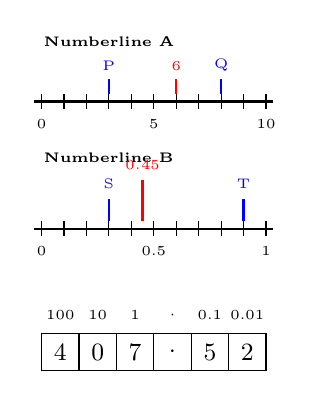
\begin{tikzpicture}[scale=0.95]

% --- Line A: 0 to 10, ticks every 1 ---
\node[font=\tiny\bfseries, anchor=west] at (-0.1,4.6) {Numberline A};
\draw[thick] (-0.1,3.8) -- (3.1,3.8);
\foreach \x in {0,0.3,0.6,0.9,1.2,1.5,1.8,2.1,2.4,2.7,3}
  \draw (\x,3.7) -- (\x,3.9);
\foreach \x/\lab in {0/0,1.5/5,3/10} \node[font=\tiny] at (\x,3.5) {\lab};
% Given points: P at 3, Q at 8. Kept low, so they stay clear of the Line A heading.
\draw[blue, thick] (0.9,3.9) -- (0.9,4.1);
\node[blue, font=\tiny] at (0.9,4.28) {P};
\draw[blue, thick] (2.4,3.9) -- (2.4,4.1);
\node[blue, font=\tiny] at (2.4,4.28) {Q};
% --- Q3 answer: 6 marked on Line A ---
\draw[ans] (1.8,3.9) -- (1.8,4.1);
\node[anslab] at (1.8,4.28) {$6$};

% --- Numberline B: 0 to 1 in tenths ---
\node[font=\tiny\bfseries, anchor=west] at (-0.1,3.05) {Numberline B};
\draw[thick] (-0.1,2.1) -- (3.1,2.1);
\foreach \x in {0,0.3,0.6,0.9,1.2,1.5,1.8,2.1,2.4,2.7,3}
  \draw (\x,2.0) -- (\x,2.2);
\foreach \x/\lab in {0/0,1.5/0.5,3/1} \node[font=\tiny] at (\x,1.8) {\lab};
% Given points: S at 0.3, T at 0.9
\draw[blue, thick] (0.9,2.2) -- (0.9,2.5);
\node[blue, font=\tiny] at (0.9,2.7) {S};
\draw[blue, thick] (2.7,2.2) -- (2.7,2.5);
\node[blue, font=\tiny] at (2.7,2.7) {T};
% --- Q3 answer: 0.45 marked on Line B, raised clear of the blue S label ---
\draw[ans] (1.35,2.2) -- (1.35,2.75);
\node[anslab] at (1.35,2.95) {$0.45$};

% --- Place value chart for 407.52 ---

\foreach \i/\head/\digit in {0/100/4,1/10/0,2/1/7,3/{$\cdot$}/{$\cdot$},4/0.1/5,5/0.01/2} {
  \draw ({0.5*\i},0.2) rectangle ({0.5*\i+0.5},0.7);
  \node[font=\tiny] at ({0.5*\i+0.25},0.95) {\head};
  \node[font=\small] at ({0.5*\i+0.25},0.45) {\digit};
}

\end{tikzpicture}
\end{center}

\column{0.70\textwidth}

\small
\begin{multicols}{2}
\begin{enumerate}\qtight

  \item On numberline A what numbers are marked by  $P$ and $Q$? \ashow{$3$ and $8$}

  \item On numberline B what numbers are marked by  $S$ and $T$? \ashow{$0.3$ and $0.9$}

  \item Mark $6$ on Line~A and $0.45$ on Line~B.

  \item Sam says $P=4$, as it is the $4$th mark. What has he done wrong? \ashow{Counted marks, not steps: $P=3$}
  \columnbreak

  \item The chart shows $407.52$. What is the $4$ worth? And the $5$? \ashow{$400$ and $0.5$}


  \item Work out $407.52\times 10$ and $407.52\div 10$. \ashow{$4075.2$ and $40.752$}

  \item A numberline goes $3.6$ to $3.7$ in $10$ equal steps. What is $3$ steps along from $3.6$? \ashow{$3.63$}

  \item Use $7$, $5$, $4$, $2$ and a decimal point to make the largest number less than $100$. \ashow{$75.42$}

\end{enumerate}
\end{multicols}

\end{columns}

\end{frame}

\begin{frame}{Worked Solution: Starter 1, Question 1}
\hypertarget{work-st1}{}
\small
\textbf{Question:} On numberline A what numbers are marked by $P$ and $Q$?

\awork{\textbf{Solution:} Numberline A runs from $0$ to $10$ with $10$ equal steps, so each step is worth $1$. \\ P is $3$ steps from $0$, so $P=3$. \\ Q is $8$ steps from $0$, so $Q=8$.}
\end{frame}

\begin{frame}{Worked Solution: Starter 1, Question 2}
\small
\textbf{Question:} On numberline B what numbers are marked by $S$ and $T$?

\awork{\textbf{Solution:} Numberline B runs from $0$ to $1$ with $10$ equal steps, so each step is worth $0.1$. \\ S is $3$ steps from $0$, so $S=0.3$. \\ T is $9$ steps from $0$, so $T=0.9$.}
\end{frame}

\begin{frame}{Worked Solution: Starter 1, Question 3}
\small
\textbf{Question:} Mark $6$ on Line A and $0.45$ on Line B.

\awork{\textbf{Solution:} Line A: $6$ is the $6$th tick from $0$ (or $6$ out of $10$ steps). \\ Line B: $0.45$ is $4.5$ tenths, so it lies halfway between the $4$th and $5$th ticks after $0$.}
\end{frame}

\begin{frame}{Worked Solution: Starter 1, Question 4}
\small
\textbf{Question:} Sam says $P=4$, as it is the $4$th mark. What has he done wrong?

\awork{\textbf{Solution:} Sam counted the marks including the zero mark as $1$. The first mark is $0$, the second is $1$, the third is $2$, and the fourth is $3$. So $P=3$. He counted marks instead of steps.}
\end{frame}

\begin{frame}{Worked Solution: Starter 1, Question 5}
\small
\textbf{Question:} The chart shows $407.52$. What is the $4$ worth? And the $5$?

\awork{\textbf{Solution:} The digit $4$ is in the hundreds column, so it is worth $4\times100=400$. \\ The digit $5$ is in the tenths column, so it is worth $5\times0.1=0.5$.}
\end{frame}

\begin{frame}{Worked Solution: Starter 1, Question 6}
\small
\textbf{Question:} Work out $407.52\times 10$ and $407.52\div 10$.

\awork{\textbf{Solution:} Multiplying by $10$ moves every digit one place to the left: $407.52\times10=4075.2$. \\ Dividing by $10$ moves every digit one place to the right: $407.52\div10=40.752$.}
\end{frame}

\begin{frame}{Worked Solution: Starter 1, Question 7}
\small
\textbf{Question:} A numberline goes $3.6$ to $3.7$ in $10$ equal steps. What is $3$ steps along from $3.6$?

\awork{\textbf{Solution:} The interval from $3.6$ to $3.7$ is $0.1$. \\ Divided into $10$ equal steps, each step is $0.1\div10=0.01$. \\ Three steps give $3\times0.01=0.03$. \\ So the number is $3.6+0.03=3.63$.}
\end{frame}

\begin{frame}{Worked Solution: Starter 1, Question 8}
\small
\textbf{Question:} Use $7$, $5$, $4$, $2$ and a decimal point to make the largest number less than $100$.

\awork{\textbf{Solution:} To make the largest number less than $100$, use the largest possible two-digit whole-number part. The digits $7$ and $5$ give $75$. \\ Put the remaining digits after the decimal point in descending order: $4$ tenths, then $2$ hundredths. \\ So the largest number is $75.42$.}
\end{frame}

%------------------------------------------------
% STARTER 2: Inequality Symbols and Ordering Decimals
%------------------------------------------------
\begin{frame}{Starter 2: Inequality Symbols \& Ordering Decimals}
\hypertarget{q-st2}{}

\vspace{-2.5em}

\begin{columns}[T]

\column{0.28\textwidth}
\vspace{5em}
\begin{center}
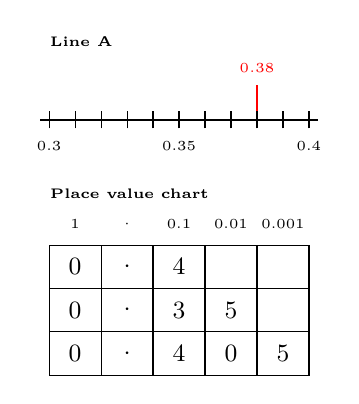
\begin{tikzpicture}[scale=1.1]

% --- Line A: 0.3 to 0.4 in hundredths ---
\node[font=\tiny\bfseries, anchor=west] at (-0.1,3.5) {Line A};
\draw[thick] (-0.1,2.6) -- (3.1,2.6);
\foreach \x in {0,0.3,0.6,0.9,1.2,1.5,1.8,2.1,2.4,2.7,3}
  \draw (\x,2.5) -- (\x,2.7);
\foreach \x/\lab in {0/0.3,1.5/0.35,3/0.4} \node[font=\tiny] at (\x,2.3) {\lab};
% --- Q5 answer: 0.38 marked ---
\draw[ans] (2.4,2.7) -- (2.4,3.0);
\node[anslab] at (2.4,3.2) {$0.38$};

% --- Place value chart: 0.4, 0.35, 0.405 ---
\node[font=\tiny\bfseries, anchor=west] at (-0.1,1.75) {Place value chart};
\foreach \i/\head in {0/1,1/{$\cdot$},2/0.1,3/0.01,4/0.001}
  \node[font=\tiny] at ({0.6*\i+0.3},1.4) {\head};
\foreach \j in {0,1,2} {
  \foreach \i in {0,1,2,3,4}
    \draw ({0.6*\i},{-0.5*\j+1.15}) rectangle ({0.6*\i+0.6},{-0.5*\j+0.65});
}
% row 1: 0.4
\foreach \i/\d in {0/0,1/{$\cdot$},2/4} \node[font=\small] at ({0.6*\i+0.3},0.9) {\d};
% row 2: 0.35
\foreach \i/\d in {0/0,1/{$\cdot$},2/3,3/5} \node[font=\small] at ({0.6*\i+0.3},0.4) {\d};
% row 3: 0.405
\foreach \i/\d in {0/0,1/{$\cdot$},2/4,3/0,4/5} \node[font=\small] at ({0.6*\i+0.3},-0.1) {\d};

\end{tikzpicture}
\end{center}

\column{0.72\textwidth}

\small
\begin{multicols}{2}
\begin{enumerate}\qtight

  \item Fill in $<$ or $>$: $7 \mathrel{\text{\ashow{$<$}}} 12$\newline $30 \mathrel{\text{\ashow{$>$}}} 3$
  \vspace{1em}

  \item In $0.405$, what is the $4$ worth? \ashow{$4$ tenths, $0.4$}

  \item On the place value chart, which is bigger, $0.4$ or $0.35$? Why? \ashow{$0.4$: $4$ tenths is greater than $3$ tenths}

  \item Fill in $<$, $>$ or $=$ $0.4 \mathrel{\text{\ashow{$=$}}} 0.40$, $0.6 \mathrel{\text{\ashow{$>$}}} 0.06$

\vspace{0.5em}

  \item Mark $0.38$ on Line A. Is it nearer $0.3$ or $0.4$? \ashow{nearer $0.4$}

  \columnbreak

  \item Order, smallest first: $0.5$, $0.45$, $0.405$, $0.54$ \ashow{$0.405$, $0.45$, $0.5$, $0.54$}

  \vspace{0.2em}

  \item True or false: more digits \emph{after} the decimal point means a bigger number? Give an example/counter-example. \ashow{False: $0.9>0.1234$}

  \vspace{0.2em}

  \item Alfie says $0.45>0.5$ as $45>5$. Explain his mistake, then write a decimal between $0.4$ and $0.405$. \ashow{$0.5$ has $5$ tenths; e.g.\ $0.402$}

\end{enumerate}
\end{multicols}

\end{columns}

\end{frame}

\begin{frame}{Worked Solution: Starter 2, Question 1}
\hypertarget{work-st2}{}
\small
\textbf{Question:} Fill in $<$ or $>$: $7 \square 12$; $30 \square 3$.

\awork{\textbf{Solution:} Compare the numbers on a number line. \\ $7$ is less than $12$, so $7<12$. \\ $30$ is greater than $3$, so $30>3$.}
\end{frame}

\begin{frame}{Worked Solution: Starter 2, Question 2}
\small
\textbf{Question:} In $0.405$, what is the $4$ worth?

\awork{\textbf{Solution:} The digits after the decimal point are tenths, hundredths, thousandths. \\ The $4$ is in the tenths column, so it is worth $4$ tenths, or $0.4$.}
\end{frame}

\begin{frame}{Worked Solution: Starter 2, Question 3}
\small
\textbf{Question:} On the place value chart, which is bigger, $0.4$ or $0.35$? Why?

\awork{\textbf{Solution:} Write both with the same number of decimal places: $0.40$ and $0.35$. \\ Compare tenths: $0.40$ has $4$ tenths, $0.35$ has $3$ tenths. \\ $4$ tenths is greater than $3$ tenths, so $0.4>0.35$.}
\end{frame}

\begin{frame}{Worked Solution: Starter 2, Question 4}
\small
\textbf{Question:} Fill in $<$, $>$ or $=$: $0.4 \square 0.40$, $0.6 \square 0.06$.

\awork{\textbf{Solution:} $0.4=0.40$ because the extra zero is in the hundredths place and does not change the value. \\ $0.6=0.60$, and $0.60$ has $60$ hundredths while $0.06$ has $6$ hundredths. So $0.6>0.06$.}
\end{frame}

\begin{frame}{Worked Solution: Starter 2, Question 5}
\small
\textbf{Question:} Mark $0.38$ on Line A. Is it nearer $0.3$ or $0.4$?

\awork{\textbf{Solution:} Line A goes from $0.3$ to $0.4$ in tenths of a hundredth, i.e. steps of $0.01$. \\ $0.38$ is $8$ steps from $0.3$, and $2$ steps from $0.4$. \\ So it is nearer $0.4$.}
\end{frame}

\begin{frame}{Worked Solution: Starter 2, Question 6}
\small
\textbf{Question:} Order, smallest first: $0.5$, $0.45$, $0.405$, $0.54$.

\awork{\textbf{Solution:} Write them with three decimal places: $0.500$, $0.450$, $0.405$, $0.540$. \\ Compare the digits: $405<450<500<540$. \\ So the order is $0.405$, $0.45$, $0.5$, $0.54$.}
\end{frame}

\begin{frame}{Worked Solution: Starter 2, Question 7}
\small
\textbf{Question:} True or false: more digits \emph{after} the decimal point means a bigger number? Give an example/counter-example.

\awork{\textbf{Solution:} False. \\ Counter-example: $0.9$ has one digit after the decimal point, while $0.1234$ has four. But $0.9=0.9000$, which is greater than $0.1234$. \\ So more digits does not always mean a bigger number.}
\end{frame}

\begin{frame}{Worked Solution: Starter 2, Question 8}
\small
\textbf{Question:} Alfie says $0.45>0.5$ as $45>5$. Explain his mistake, then write a decimal between $0.4$ and $0.405$.

\awork{\textbf{Solution:} Alfie compared $45$ and $5$ as whole numbers. But $0.45$ means $45$ hundredths, while $0.5$ means $5$ tenths $=0.50=50$ hundredths. \\ Since $45<50$, we have $0.45<0.5$. \\ A decimal between $0.4$ and $0.405$ is $0.402$ (or $0.401$, $0.403$, $0.404$).}
\end{frame}

%------------------------------------------------
% STARTER 3: Negative Numbers
%------------------------------------------------
\begin{frame}{Starter 3: Ordering Negative Numbers}
\hypertarget{q-st3}{}

\vspace{-2.5em}

\begin{columns}[T]

\column{0.30\textwidth}
\begin{center}
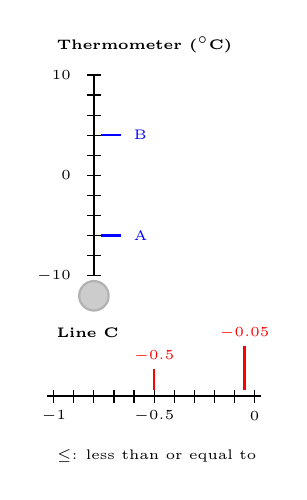
\begin{tikzpicture}[scale=0.85]

% --- Thermometer: -10 to 10, one tick every 2 degrees, only -10/0/10 labelled ---
\node[font=\tiny\bfseries, anchor=west] at (-0.1,3.45) {Thermometer ($^\circ$C)};
\draw[thick] (0.6,0) -- (0.6,3);
\foreach \y in {0,0.3,0.6,0.9,1.2,1.5,1.8,2.1,2.4,2.7,3}
  \draw (0.5,\y) -- (0.7,\y);
\foreach \y/\lab in {0/{$-10$},1.5/{$0$},3/{$10$}}
  \node[font=\tiny, anchor=east] at (0.4,\y) {\lab};
\fill[gray!40] (0.6,-0.3) circle (0.22);
\draw[gray!60, thick] (0.6,-0.3) circle (0.22);
% Given readings: A at -6, B at 4 (both sit exactly on a tick)
\draw[blue, thick] (0.7,0.6) -- (1.0,0.6);
\node[blue, font=\tiny, anchor=west] at (1.05,0.6) {A};
\draw[blue, thick] (0.7,2.1) -- (1.0,2.1);
\node[blue, font=\tiny, anchor=west] at (1.05,2.1) {B};

% --- Line C: -1 to 0 in tenths ---
\node[font=\tiny\bfseries, anchor=west] at (-0.1,-0.85) {Line C};
\draw[thick] (-0.1,-1.8) -- (3.1,-1.8);
\foreach \x in {0,0.3,0.6,0.9,1.2,1.5,1.8,2.1,2.4,2.7,3}
  \draw (\x,-1.9) -- (\x,-1.7);
\foreach \x/\lab in {0/{$-1$},1.5/{$-0.5$},3/{$0$}} \node[font=\tiny] at (\x,-2.1) {\lab};
% Reminder for the challenge question, which is the deck's only use of a weak inequality
\node[font=\tiny, anchor=west] at (-0.1,-2.7) {$\leq$: less than or equal to};
% --- Q5 answers: -0.5 and -0.05 marked on Line C, at different heights ---
\draw[ans] (1.5,-1.7) -- (1.5,-1.4);
\node[anslab] at (1.5,-1.2) {$-0.5$};
\draw[ans] (2.85,-1.7) -- (2.85,-1.05);
\node[anslab] at (2.85,-0.85) {$-0.05$};

\end{tikzpicture}
\end{center}

\column{0.70\textwidth}

\small
\begin{multicols}{2}
\begin{enumerate}\qtight

  \item Which is colder, $4\,^\circ$C or $-4\,^\circ$C? \ashow{$-4\,^\circ$C}

  \item What is each mark on the thermometer worth? Write the temperatures at A and B. \ashow{$2\,^\circ$C per mark; A $=-6$, B $=4$}

  \item Which is colder, $-3$ or $-8$? Fill in: $-3 \mathrel{\text{\ashowq{$>$}}} -8$ \ashow{($-8$ is colder)}

  \item Order, smallest first: $-2$, $5$, $-7$, $0$, $-1$ \ashow{($-7,-2,-1,0,5$)}

  \columnbreak

  \item Mark $-0.5$ and $-0.05$ on Line C. Which is larger? \ashow{$-0.05$}

  \item Fill in $<$ or $>$: $-4.5 \mathrel{\text{\ashowq{$<$}}} -4.05$, $-0.3 \mathrel{\text{\ashowq{$<$}}} 0.03$

  \item (Extension) Order, smallest first: $-0.08$, $0.7$, $-0.8$, $-0.75$ \ashow{($-0.8$, $-0.75$, $-0.08$, $0.7$)}

  \item (Challenge) List the integers $n$: $-3\leq n<2$. Write a number between $-0.5$ and $-0.4$. \ashow{$-3,-2,-1,0,1$; e.g.\ $-0.45$}

\end{enumerate}
\end{multicols}

\end{columns}

\end{frame}

\begin{frame}{Worked Solution: Starter 3, Question 1}
\hypertarget{work-st3}{}
\small
\textbf{Question:} Which is colder, $4\,^\circ$C or $-4\,^\circ$C?

\awork{\textbf{Solution:} Negative temperatures are below zero. \\ $-4\,^\circ$C is $4$ degrees below zero, while $4\,^\circ$C is $4$ degrees above zero. \\ So $-4\,^\circ$C is colder.}
\end{frame}

\begin{frame}{Worked Solution: Starter 3, Question 2}
\small
\textbf{Question:} What is each mark on the thermometer worth? Write the temperatures at A and B.

\awork{\textbf{Solution:} The thermometer goes from $-10$ to $10$, with $10$ equal intervals. \\ The total range is $20\,^\circ$C, so each mark is $20\div10=2\,^\circ$C. \\ A is $2$ marks above $-10$, so A $=-10+2\times2=-6\,^\circ$C. \\ B is $2$ marks above $0$, so B $=0+2\times2=4\,^\circ$C.}
\end{frame}

\begin{frame}{Worked Solution: Starter 3, Question 3}
\small
\textbf{Question:} Which is colder, $-3$ or $-8$? Fill in: $-3 \square -8$.

\awork{\textbf{Solution:} On a number line, $-8$ is further left than $-3$. \\ So $-8$ is colder. \\ Since $-3$ is to the right of $-8$, we have $-3>-8$. \\ Fill in $>$.}
\end{frame}

\begin{frame}{Worked Solution: Starter 3, Question 4}
\small
\textbf{Question:} Order, smallest first: $-2$, $5$, $-7$, $0$, $-1$.

\awork{\textbf{Solution:} Negative numbers are less than $0$ and less than positive numbers. \\ Order the negatives: $-7<-2<-1$. \\ Then $0$, then $5$. \\ So the order is $-7$, $-2$, $-1$, $0$, $5$.}
\end{frame}

\begin{frame}{Worked Solution: Starter 3, Question 5}
\small
\textbf{Question:} Mark $-0.5$ and $-0.05$ on Line C. Which is larger?

\awork{\textbf{Solution:} Line C goes from $-1$ to $0$. \\ $-0.5$ is halfway between $-1$ and $0$. \\ $-0.05$ is very close to $0$. \\ On the number line, $-0.05$ is to the right of $-0.5$, so $-0.05$ is larger.}
\end{frame}

\begin{frame}{Worked Solution: Starter 3, Question 6}
\small
\textbf{Question:} Fill in $<$ or $>$: $-4.5 \square -4.05$, $-0.3 \square 0.03$.

\awork{\textbf{Solution:} $-4.5$ is further left than $-4.05$, so $-4.5<-4.05$. \\ $-0.3$ is negative and $0.03$ is positive, so $-0.3<0.03$.}
\end{frame}

\begin{frame}{Worked Solution: Starter 3, Question 7}
\small
\textbf{Question:} (Extension) Order, smallest first: $-0.08$, $0.7$, $-0.8$, $-0.75$.

\awork{\textbf{Solution:} Compare the negative decimals first. \\ $-0.8<-0.75<-0.08$. \\ The only positive number is $0.7$, which is largest. \\ So the order is $-0.8$, $-0.75$, $-0.08$, $0.7$.}
\end{frame}

\begin{frame}{Worked Solution: Starter 3, Question 8}
\small
\textbf{Question:} (Challenge) List the integers $n$: $-3\leq n<2$. Write a number between $-0.5$ and $-0.4$.

\awork{\textbf{Solution:} The integers from $-3$ up to but not including $2$ are $-3$, $-2$, $-1$, $0$, $1$. \\ A number between $-0.5$ and $-0.4$ is $-0.45$ (or $-0.42$, etc.).}
\end{frame}

%------------------------------------------------
% STARTER 4: Rounding Integers
%------------------------------------------------
\begin{frame}{Starter 4: Rounding Integers}
\hypertarget{q-st4}{}

\vspace{-2.5em}

\begin{columns}[T]

\column{0.30\textwidth}
\begin{center}
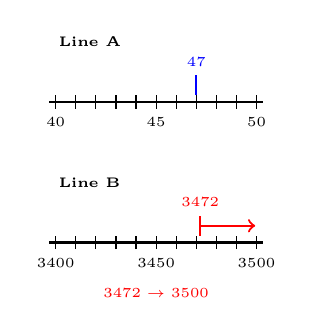
\begin{tikzpicture}[scale=0.85]

% --- Line A: 40 to 50, ticks every 1 ---
\node[font=\tiny\bfseries, anchor=west] at (-0.1,3.5) {Line A};
\draw[thick] (-0.1,2.6) -- (3.1,2.6);
\foreach \x in {0,0.3,0.6,0.9,1.2,1.5,1.8,2.1,2.4,2.7,3}
  \draw (\x,2.5) -- (\x,2.7);
\foreach \x/\lab in {0/40,1.5/45,3/50} \node[font=\tiny] at (\x,2.3) {\lab};
% Given point: 47
\draw[blue, thick] (2.1,2.7) -- (2.1,3.0);
\node[blue, font=\tiny] at (2.1,3.2) {$47$};

% --- Line B: 3400 to 3500, ticks every 10 ---
\node[font=\tiny\bfseries, anchor=west] at (-0.1,1.4) {Line B};
\draw[thick] (-0.1,0.5) -- (3.1,0.5);
\foreach \x in {0,0.3,0.6,0.9,1.2,1.5,1.8,2.1,2.4,2.7,3}
  \draw (\x,0.4) -- (\x,0.6);
\foreach \x/\lab in {0/3400,1.5/3450,3/3500} \node[font=\tiny] at (\x,0.2) {\lab};
% --- Q4 answers: 3472 marked, with an arrow to the nearer end ---
\draw[ans] (2.16,0.6) -- (2.16,0.9);
\node[anslab] at (2.16,1.1) {$3472$};
\draw[ans, ->] (2.16,0.75) -- (2.98,0.75);
\node[anslab] at (1.5,-0.25) {$3472 \to 3500$};

\end{tikzpicture}
\end{center}

\column{0.70\textwidth}

\small
\begin{multicols}{2}
\begin{enumerate}\qtight

  \item Fill in $<$ or $>$: $-6 \mathrel{\text{\ashowq{$<$}}} -2$

  \item Line A: is $47$ nearer $40$ or $50$? Round it to the nearest $10$. \ashow{nearer $50$, so $50$}

  \item Round to the nearest $10$: $32$, $85$ \ashow{($30$ and $90$)}

  \item Mark $3472$ on Line B, then round it to the nearest $100$.

  \item Round $3472$ to the nearest $10$; to the nearest $1000$. \ashow{$3470$ and $3000$}

  \columnbreak

  \item Round $4950$ to the nearest $100$. \ashow{$5000$}

  \item (Extension) Zoe rounds $8449$ to the nearest $100$: $8449\to 8450\to 8500$. What is her mistake? \ashow{Rounded twice: only the tens digit $4$ counts, so $8400$}

  \item (Challenge) A number rounds to $250$ to the nearest $10$. Smallest it could be? Largest? \ashow{$245$ and $254$}

\end{enumerate}
\end{multicols}

\end{columns}

\end{frame}

\begin{frame}{Worked Solution: Starter 4, Question 1}
\hypertarget{work-st4}{}
\small
\textbf{Question:} Fill in $<$ or $>$: $-6 \square -2$.

\awork{\textbf{Solution:} On a number line, $-6$ is to the left of $-2$. \\ So $-6$ is less than $-2$. \\ Therefore $-6<-2$.}
\end{frame}

\begin{frame}{Worked Solution: Starter 4, Question 2}
\small
\textbf{Question:} Line A: is $47$ nearer $40$ or $50$? Round it to the nearest $10$.

\awork{\textbf{Solution:} $47$ is $7$ away from $40$ and $3$ away from $50$. \\ So it is nearer $50$. \\ To the nearest $10$, $47$ rounds to $50$.}
\end{frame}

\begin{frame}{Worked Solution: Starter 4, Question 3}
\small
\textbf{Question:} Round to the nearest $10$: $32$, $85$.

\awork{\textbf{Solution:} For $32$, the ones digit is $2$, which is less than $5$, so round down to $30$. \\ For $85$, the ones digit is $5$, so round up to $90$.}
\end{frame}

\begin{frame}{Worked Solution: Starter 4, Question 4}
\small
\textbf{Question:} Mark $3472$ on Line B, then round it to the nearest $100$.

\awork{\textbf{Solution:} Line B goes from $3400$ to $3500$. \\ $3472$ is $72$ from $3400$ and $28$ from $3500$, so it is nearer $3500$. \\ To round to the nearest $100$, look at the tens digit, which is $7$. Since $7\geq5$, round up. \\ So $3472$ rounds to $3500$.}
\end{frame}

\begin{frame}{Worked Solution: Starter 4, Question 5}
\small
\textbf{Question:} Round $3472$ to the nearest $10$; to the nearest $1000$.

\awork{\textbf{Solution:} Nearest $10$: look at the ones digit, $2$. Since $2<5$, round down to $3470$. \\ Nearest $1000$: look at the hundreds digit, $4$. Since $4<5$, round down to $3000$.}
\end{frame}

\begin{frame}{Worked Solution: Starter 4, Question 6}
\small
\textbf{Question:} Round $4950$ to the nearest $100$.

\awork{\textbf{Solution:} To round to the nearest $100$, look at the tens digit, which is $5$. \\ Since $5\geq5$, round up. \\ $4950$ rounds to $5000$.}
\end{frame}

\begin{frame}{Worked Solution: Starter 4, Question 7}
\small
\textbf{Question:} (Extension) Zoe rounds $8449$ to the nearest $100$: $8449\to 8450\to 8500$. What is her mistake?

\awork{\textbf{Solution:} Zoe rounded twice. \\ To round $8449$ to the nearest $100$, look only at the tens digit, which is $4$. \\ Since $4<5$, round down. \\ So $8449$ rounds to $8400$, not $8500$.}
\end{frame}

\begin{frame}{Worked Solution: Starter 4, Question 8}
\small
\textbf{Question:} (Challenge) A number rounds to $250$ to the nearest $10$. Smallest it could be? Largest?

\awork{\textbf{Solution:} Numbers that round to $250$ to the nearest $10$ lie from halfway below $250$ to halfway above $250$. \\ Halfway below is $245$, and halfway above is $255$. \\ Since $255$ would round to $260$, the largest is $254$. \\ So the smallest is $245$ and the largest is $254$.}
\end{frame}

%------------------------------------------------
% STARTER 5: Rounding Decimals, Recurring and Irrational
%------------------------------------------------
\begin{frame}{Starter 5: Rounding Decimals \& Never-Ending Decimals}
\hypertarget{q-st5}{}

\vspace{-2.5em}

\begin{columns}[T]

\column{0.30\textwidth}
\begin{center}
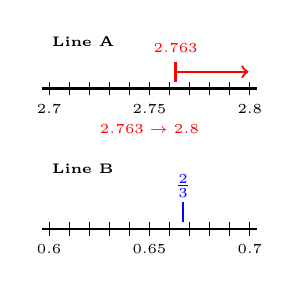
\begin{tikzpicture}[scale=0.85]

% --- Line A: 2.7 to 2.8 in hundredths ---
% Heading sits at 3.3 rather than 3.5: this frame's title is two lines' worth of
% width and the diagram column otherwise crowds it.
\node[font=\tiny\bfseries, anchor=west] at (-0.1,3.3) {Line A};
\draw[thick] (-0.1,2.6) -- (3.1,2.6);
\foreach \x in {0,0.3,0.6,0.9,1.2,1.5,1.8,2.1,2.4,2.7,3}
  \draw (\x,2.5) -- (\x,2.7);
\foreach \x/\lab in {0/2.7,1.5/2.75,3/2.8} \node[font=\tiny] at (\x,2.3) {\lab};
% (the Line A heading sits low here, to keep clear of the frame title)
% --- Q3 answers: 2.763 marked, with an arrow to the nearer end ---
\draw[ans] (1.89,2.7) -- (1.89,3.0);
\node[anslab] at (1.89,3.2) {$2.763$};
\draw[ans, ->] (1.89,2.85) -- (2.98,2.85);
\node[anslab] at (1.5,2.0) {$2.763 \to 2.8$};

% --- Line B: 0.6 to 0.7 in hundredths, with 2/3 shown ---
\node[font=\tiny\bfseries, anchor=west] at (-0.1,1.4) {Line B};
\draw[thick] (-0.1,0.5) -- (3.1,0.5);
\foreach \x in {0,0.3,0.6,0.9,1.2,1.5,1.8,2.1,2.4,2.7,3}
  \draw (\x,0.4) -- (\x,0.6);
\foreach \x/\lab in {0/0.6,1.5/0.65,3/0.7} \node[font=\tiny] at (\x,0.2) {\lab};
% Given point: 2/3 = 0.6666...
\draw[blue, thick] (2.0,0.6) -- (2.0,0.9);
\node[blue, font=\scriptsize] at (2.0,1.15) {$\tfrac{2}{3}$};

\end{tikzpicture}

\vspace{0.4em}
{\scriptsize
\begin{tabular}{@{}l@{}}
\textbf{Never-ending decimals} \\[0.15em]
$\frac{2}{3} = 0.6666\ldots = 0.\dot{6}$ \\
$\frac{1}{7} = 0.142857142857\ldots$ \\
$\pi = 3.14159265\ldots$ \\
$\sqrt{2} = 1.41421356\ldots$ \\
$0.1010010001\ldots$
\end{tabular}}
\end{center}

\column{0.70\textwidth}

\small
\begin{multicols}{2}
\begin{enumerate}\qtight

  \item Round $4738$ to the nearest $100$. \ashow{$4700$}

  \item Round to the nearest whole number: $4.6$, $12.348$ \ashow{($5$ and $12$)}

  \item Mark $2.763$ on Line A. Round it to $1$ decimal place (d.p.).

  \item Round to $1$ d.p.: $4.62$, $0.95$. Why is $0.95$ not $1$? \ashow{$4.6$, $1.0$ --- $1$ d.p.\ needs one decimal digit}

  \item Round $12.348$ to $2$ d.p., then to $1$ d.p. Why not $12.4$? \ashow{$12.35$, $12.3$ --- never round twice}

  \columnbreak

  \item Line B shows $\frac{2}{3}=0.\dot{6}$. Round it to $1$ d.p.\ and $2$ d.p. \ashow{$0.7$ and $0.67$}

  \item (Extension) Write $\frac{1}{3}$ in dot notation, then round $\frac{1}{7}$ to $3$ d.p. \ashow{$0.\dot{3}$ and $0.143$}

  \item (Challenge) Which listed decimals never settle into a repeating block? Can one still be a fraction? \ashow{$\pi$, $\sqrt{2}$, $0.101001\ldots$; yes: $0.\dot{3}=\frac13$}

\end{enumerate}
\end{multicols}

\end{columns}

\end{frame}

\begin{frame}{Worked Solution: Starter 5, Question 1}
\hypertarget{work-st5}{}
\small
\textbf{Question:} Round $4738$ to the nearest $100$.

\awork{\textbf{Solution:} To round to the nearest $100$, look at the tens digit. \\ In $4738$, the tens digit is $3$. \\ Since $3<5$, round down. \\ So $4738$ rounds to $4700$.}
\end{frame}

\begin{frame}{Worked Solution: Starter 5, Question 2}
\small
\textbf{Question:} Round to the nearest whole number: $4.6$, $12.348$.

\awork{\textbf{Solution:} For $4.6$, look at the tenths digit, $6$. Since $6\geq5$, round up to $5$. \\ For $12.348$, look at the tenths digit, $3$. Since $3<5$, round down to $12$.}
\end{frame}

\begin{frame}{Worked Solution: Starter 5, Question 3}
\small
\textbf{Question:} Mark $2.763$ on Line A. Round it to $1$ decimal place (d.p.).

\awork{\textbf{Solution:} Line A goes from $2.7$ to $2.8$. $2.763$ is between $2.76$ and $2.77$, closer to $2.8$. \\ To round to $1$ d.p., look at the hundredths digit, which is $6$. \\ Since $6\geq5$, round the tenths digit $7$ up to $8$. \\ So $2.763$ rounds to $2.8$.}
\end{frame}

\begin{frame}{Worked Solution: Starter 5, Question 4}
\small
\textbf{Question:} Round to $1$ d.p.: $4.62$, $0.95$. Why is $0.95$ not $1$?

\awork{\textbf{Solution:} $4.62$ to $1$ d.p.: the hundredths digit is $2$, so round down to $4.6$. \\ $0.95$ to $1$ d.p.: the hundredths digit is $5$, so round up. The tenths digit $9$ becomes $10$, which carries to give $1.0$. \\ It is not written as $1$ because $1$ d.p. requires one digit after the decimal point.}
\end{frame}

\begin{frame}{Worked Solution: Starter 5, Question 5}
\small
\textbf{Question:} Round $12.348$ to $2$ d.p., then to $1$ d.p. Why not $12.4$?

\awork{\textbf{Solution:} To $2$ d.p.: look at the thousandths digit, $8$. Since $8\geq5$, round up to $12.35$. \\ To $1$ d.p.: start again from $12.348$. Look at the hundredths digit, $4$. Since $4<5$, round down to $12.3$. \\ It is not $12.4$ because you must not round the already rounded $12.35$ again.}
\end{frame}

\begin{frame}{Worked Solution: Starter 5, Question 6}
\small
\textbf{Question:} Line B shows $\frac{2}{3}=0.\dot{6}$. Round it to $1$ d.p. and $2$ d.p.

\awork{\textbf{Solution:} $\frac{2}{3}=0.6666\ldots$. \\ To $1$ d.p.: the hundredths digit is $6$, so round up to $0.7$. \\ To $2$ d.p.: the thousandths digit is $6$, so round up to $0.67$.}
\end{frame}

\begin{frame}{Worked Solution: Starter 5, Question 7}
\small
\textbf{Question:} (Extension) Write $\frac{1}{3}$ in dot notation, then round $\frac{1}{7}$ to $3$ d.p.

\awork{\textbf{Solution:} $\frac{1}{3}=0.3333\ldots$, so in dot notation it is $0.\dot{3}$. \\ $\frac{1}{7}=0.142857142857\ldots$. \\ To $3$ d.p., look at the fourth decimal digit. The digits are $1$, $4$, $2$, $8$, so the fourth digit is $8$. \\ Since $8\geq5$, round the third digit $2$ up to $3$. \\ So $\frac{1}{7}\approx0.143$.}
\end{frame}

\begin{frame}{Worked Solution: Starter 5, Question 8}
\small
\textbf{Question:} (Challenge) Which listed decimals never settle into a repeating block? Can one still be a fraction?

\awork{\textbf{Solution:} The listed decimals that never settle into a repeating block are $\pi$, $\sqrt{2}$, and $0.1010010001\ldots$. \\ These are irrational, so they cannot be written as fractions. \\ However, a never-ending decimal that does repeat can be a fraction, e.g. $0.\dot{3}=\frac{1}{3}$.}
\end{frame}

\end{document}